\documentclass[11pt]{article}

\usepackage[top=1.25in, bottom=1.25in, left=1.75in, right=1.75in]{geometry}
% \def\changemargin#1#2{\list{}{\rightmargin#2\leftmargin#1}\item[]}
% \let\endchangemargin=\endlist
\usepackage{abstract}
\usepackage{amsmath}
\usepackage{graphicx}
\renewcommand{\abstractname}{}  
\usepackage[document]{ragged2e}
\usepackage{listings}
\usepackage{pgfplots}
\usepackage{url}
\usepackage{tikz}
\usetikzlibrary{datavisualization}
\usetikzlibrary{datavisualization.formats.functions}
\usetikzlibrary{backgrounds}
\newcommand*\circled[1]{\tikz[baseline=(char.base)]{
            \node[shape=circle,draw,inner sep=2pt] (char) {#1};}}

\title{\textbf{Expanding the Hakaru language to investigate probabilistic program transformation}}
\author{Justin Staples, Mahmoud Khattab, Nevin Mahilal, Arian Sohrabi}

\begin{document}

\maketitle

%%%%%%%%%%%%%%%%%%%%%%%%%%%%%%%%%%%%%%%%%%%%%%%%%%%%%%%%%%%%%%%%%%%%
% Abstract
%%%%%%%%%%%%%%%%%%%%%%%%%%%%%%%%%%%%%%%%%%%%%%%%%%%%%%%%%%%%%%%%%%%%

\begin{abstract}
% \begin{changemargin}{0.5in}{0.5in}
\noindent
\begin{justify}
\textbf{Abstract.} We present our work on Hakaru, a probabilistic programming language that has been expanded with the addition of new features and built in functions. Development on this project can be divided into two major endeavours. First, we present a strategy for developing implementations of new statistical distributions using the primitives that already existed in Hakaru. Known relationships between distributions are then used to test the validity of the Hakaru language. A small subset of the newly added disbributions have been tested in this way with mostly failing results. 
\end{justify}
\end{abstract}
% \end{changemargin} 

%%%%%%%%%%%%%%%%%%%%%%%%%%%%%%%%%%%%%%%%%%%%%%%%%%%%%%%%%%%%%%%%%%%%
% Introduction
%%%%%%%%%%%%%%%%%%%%%%%%%%%%%%%%%%%%%%%%%%%%%%%%%%%%%%%%%%%%%%%%%%%%

\section{Introduction}

\begin{justify}

Often, we wish to create a model for some kind of real world phenomenon so that we can extract useful information and learn more about it. For example, in a machine learning application, the goal is often to predict or infer information about the model based on the past outcomes of some kind of experiment. An experiment could result in many different outcomes, each one with a different likelihood (probability).

The mathematical functions that we use to describe these probabilties are called probability distributions and the quantity that denotes the outcome of the experiment is called a random variable. A random variable can take on continuous or discrete values depending on the application. Continuous random variables are formally defined by a probability density function (PDF), which maps the outcomes of the random variable to real numbers that represent a probability. Similarly, a discrete random variable is described by a probability mass function (PMF). As an example, consider one of the most ubiquitous and naturally occuring distributions, the normal distribution. We can say that a random variable, \textit{X}, is normally distributed with the following notation.

\begin{center}
\boxed{\textit{X} \sim Normal(\mu, \sigma^2)}
\end{center}

Here, we can see that the normal distribution is parametrized by $\mu$, the population mean, and $\sigma$, the standard deviation. A plot the PDF is shown below. Remember that the PDF describes the liklihood that a value sampled from this distribution will equal $x$.

\begin{figure}[h]
\centering
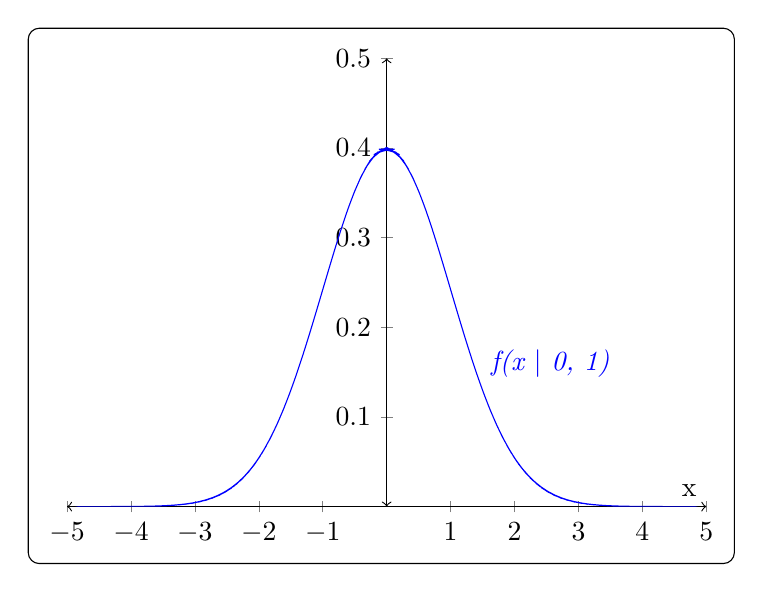
\begin{tikzpicture}[framed, style={rounded corners}][>=stealth]
    \begin{axis}[
        xmin=-5,xmax=5,
        xtick={-5,-4,-3,-2,-1,0,1,2,3,4,5},
        xlabel=x,
        ymin=0,ymax=0.5,
        axis x line=middle,
        axis y line=middle,
        axis line style=<->,
    	width=0.8*\textwidth,
        height=\axisdefaultheight
        ]
        \addplot[no marks,blue,-] expression[domain=-5:5,samples=100]{1/sqrt(2*pi)*exp(-x^2/2)} 
                    node[pos=0.65,anchor=south west]{\textit{f(x $\mid$ 0, 1)}}; 
    \end{axis}
\end{tikzpicture}
\caption{PDF of the normal distribution, with $\mu = 0$ and $\sigma = 1$}
\end{figure}

Hakaru \cite{narayanan2016probabilistic} is an experimental probabilistic programming language (PPL) which allows users to create probabilistic models (implementations of statistical distributions). Running a Hakaru program generates a stream of random numbers (known as samples) distributed according to the distribution defined in the program code. The language is quite small given its specialized domain. However, Hakaru programs can be compiled to C and Haskell, making for an easy way to export probabilistic models defined in Hakaru into imperative and functional programming domains. These can then be used within larger applications (e.g. simulating scenarios with inherent uncertainty, generating training sets for machine learning algorithms).

The purpose of Hakaru is to simplify the process of implementing efficient probabilistic models. The small size of the language solves the problem of simplifying model implementation. In order to simplify the process of making these implementations efficient, Hakaru includes some inference algorithms that transform Hakaru programs into other forms. Most pertinent to our project is {\tt hk-maple} (formerly known as {\tt simplify}). In short, {\tt hk-maple} takes a Hakaru program file as an argument and uses Maple to perform algebraic transformations. If the simplify mode of {\tt hk-maple} is used (the default mode), it returns an equivalent Hakaru program with greater sampling efficiency. In applications which may require billions of samplings, such as machine learning, this has the potential to save a significant amount of processing time.


\end{justify}

%%%%%%%%%%%%%%%%%%%%%%%%%%%%%%%%%%%%%%%%%%%%%%%%%%%%%%%%%%%%%%%%%%%%
% Motivation
%%%%%%%%%%%%%%%%%%%%%%%%%%%%%%%%%%%%%%%%%%%%%%%%%%%%%%%%%%%%%%%%%%%%

\section{Motivation}

\begin{justify}

As a probabilistic programming language, Hakaru is well suited for machine learning applications and problems that have inherent uncertainty. The workflow of many of these problems have elements in common. Hakaru was originally designed with ease of use in mind, meaning that it aims to streamline the process of designing solutions for these types of problems. The system description of Hakaru presents a new, modular approach to designing these solutions such that the solutions can be reused and composed with others. Studying the nature of the Hakaru language can reveal useful information about how these probabilistic models can be used to solve problems. 

The purpose of our project is two-fold. Our first objective is to increase the accessibility to Hakaru for future users. Our main effort in this regard has been the development of a standard library in which we have implemented over 60 statistical distributions which cover a wide range of potential applications. Another effort to increase accessibility has been the development of a syntax highlighting package for Sublime Text; the only one currently implemented for a GUI text editor. This package has been invaluable in increasing code readability/writability, and optimizing our workflow. Lastly, a few primitive mathematical functions have been newly incorporated in to the language (e.g. {\tt choose}, {\tt log}, {\tt sin}, etc.). 

Our second objective is to test the validity of the Hakaru language. Our focus is on writing test cases based on well-known relationships between the various distributions implemented in the Standard Library. In general, our test cases transform two related distributions so that the resulting distributions are (hypothetically) equivalent to each other. The number of possible test cases we could write in this vein is beyond the scope of this project. To this end, we have focused our testing on a few distributions, with the intention of laying down the groundwork for future testing in this area.

\end{justify}

%%%%%%%%%%%%%%%%%%%%%%%%%%%%%%%%%%%%%%%%%%%%%%%%%%%%%%%%%%%%%%%%%%%%
% Related Works
%%%%%%%%%%%%%%%%%%%%%%%%%%%%%%%%%%%%%%%%%%%%%%%%%%%%%%%%%%%%%%%%%%%%

\section{Related Works}

\justifying
One of the major focuses of our project has been on testing relationships between distributions. Our team has been adding our testing files to a large testing suite written in Haskell (namely {\tt RoundTrip.hs}, where all the tests are organized). This file included hundreds of tests, many of which were written by other Hakaru developers! So, this gives evidence that these types of program transformations have been investigated before. Of course, this work is very related and relelvant to our own. As a result, we have used the structure and style of other testing files as a basis for our own. 

Although it is not known exactly if other groups are currently investigating these probabilistic program transformations in the same way as we are, probabilistic programming has been around for some time and so there are many other active projects in this domain. 

One pattern for designing probabilistic languages is to embed them in a host language. For example, the language of Hakaru is embedded in Haskell. One such other example of this pattern is WebPPL \cite{dippl}, which is a small probabilistic programming language embedded in JavaScript. There is plenty of future work to be done in terms of making efforts to implement PPLs using various other languages. 

%%%%%%%%%%%%%%%%%%%%%%%%%%%%%%%%%%%%%%%%%%%%%%%%%%%%%%%%%%%%%%%%%%%%
% Standard Library Development
%%%%%%%%%%%%%%%%%%%%%%%%%%%%%%%%%%%%%%%%%%%%%%%%%%%%%%%%%%%%%%%%%%%%

\section{Standard Library Development}

\justifying
As discussed earlier, one of our major contributions has been the addition of over 60 new probabilistic models. At the onset of the project, the Hakaru language offered a small set of simple, primitive distributions. We have greatly expanded this library of distributions so that more complex models can be easily created.

Whenever possible, we have implemented distributions as transformations on pre-existing models, starting with the primitive distributions that are native to Hakaru ({\tt normal}, {\tt categorical}, etc.). We have used the UDR (Univariate Distribution Relationship) \cite{leemis} to guide the development of the standard library, as it reveals many useful relationships bewteen relevant distributions (see Figure 2). In the case of multiple possible implementations for a distribution, we have opted for the implementation which adopts the shortest path from a primitive distribution on the UDR.

In the UDR, an arrow from distribution A to distribution B shows the transformation that must be applied to A to result in B. So, new distributions are created by combining and transforming what has already been built.

\begin{figure}
\centering
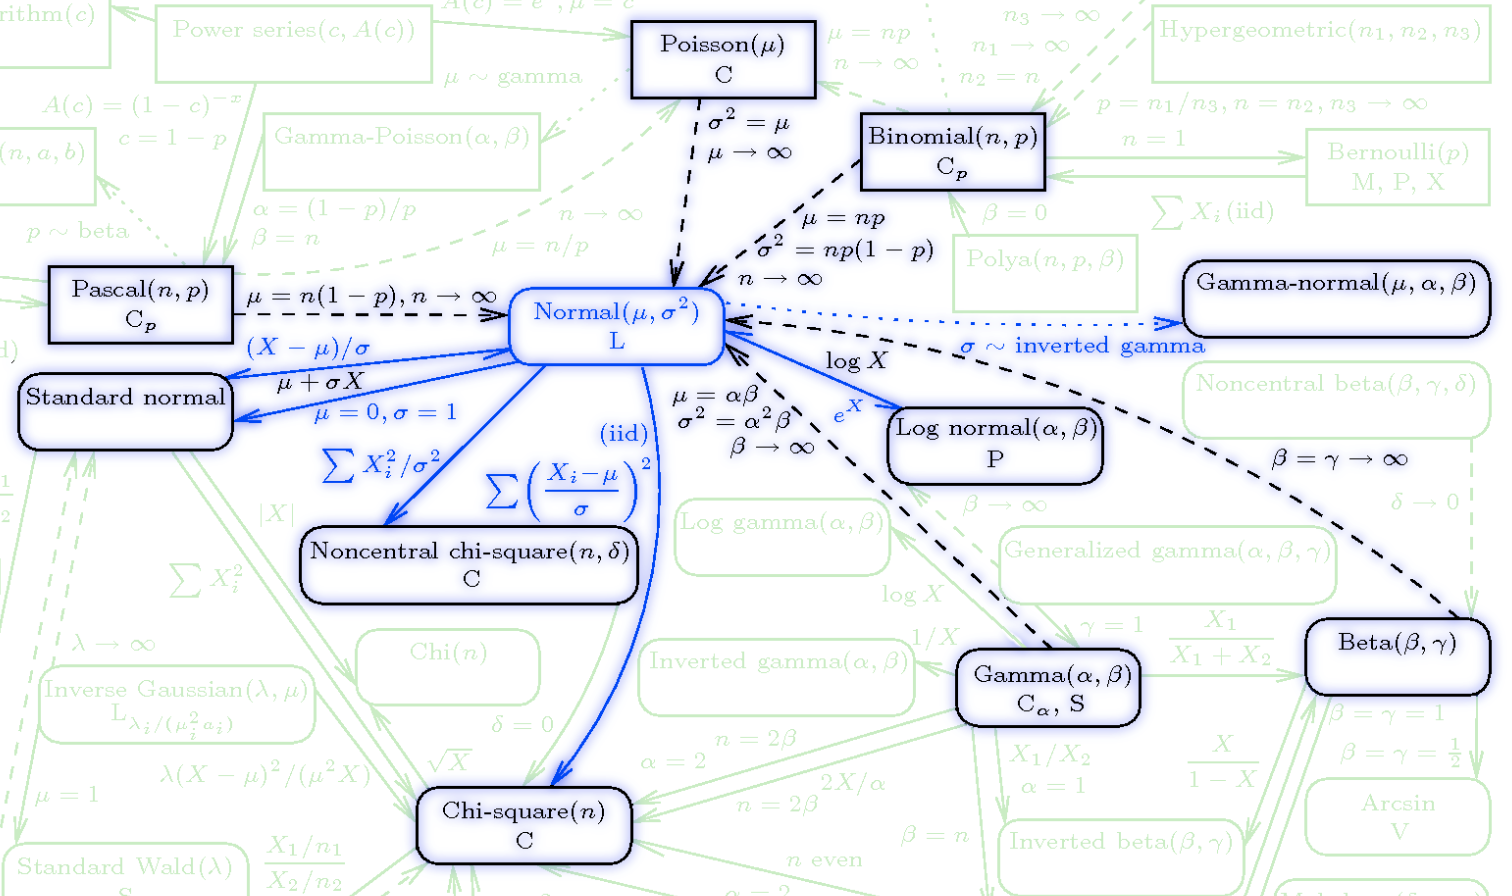
\includegraphics[height=6cm]{UDR.png}
\caption{A snapshot of the UDR shows how the normal distribution can be transformed into a multitude of other distributions.}
\end{figure}

Hakaru functions representing probabilistic models (i.e. functions with a {\tt measure(<type>)} return type) cannot be used as operands in normal mathematical operations. This is to say we cannot transform models directly (i.e. we can’t do algebraic transformation on the PDF). The only operator we can use on a model is bind ({\tt \tiny{<$\sim$}}), to pull a sample from it. However, we are able to transform samples however we like. Therefore, we are interested in implementing transformations of the following form.

\begin{center}
\boxed{R(p, q) \Rightarrow \textit{X} \sim A(p) \Rightarrow \textit{f(X)} \sim B(q)}
\end{center}

In the equation above, \textit{p} is a set of values parameterizing the distribution \textit{A}, \textit{q} is a set of values parameterizing the distribution \textit{B}, \textit{R(p, q)} is a set of relationships between \textit{p} and \textit{q} that must be satisfied, and \textit{f} is a function that applies a transformation to a sample. We can expand this definition to include transformations defined in terms of an aggregation of multiple independent samples. For example, the standard chi-square distribution is defined as the sum of the squares of \textit{n} standard normal random variables.

Hakaru also lends itself very well to Bayesian transformations where we want to pull a sample from a distribution which is parameterized with a value sampled from another distribution. These transformations take the following form. Here, we are saying that if \textit{X} is parameterized by \textit{p}, then the distribution \textit{C}, which is parameterized by \textit{p} and \textit{q}, is equal to another distribution, \textit{Y}, which is parameterized by \textit{q} and \textit{X}.

\begin{center}
\boxed{X \sim A(p) \Rightarrow Y \sim B(q, X) = C(p, q)}
\end{center}

Some distributions on the UDR are unreachable from Hakaru's primitive distributions using transformations like the 2 described above. In these cases, we have to implement the model in terms of the PMF for a discrete distribution or in terms of the PDF for a continuous distribution.


%%%%%%%%%%%%%%%%%%%%%%%%%%%%%%%%%%%%%%%%%%%%%%%%%%%%%%%%%%%%%%%%%%%%
% Testing
%%%%%%%%%%%%%%%%%%%%%%%%%%%%%%%%%%%%%%%%%%%%%%%%%%%%%%%%%%%%%%%%%%%%

\section{Testing}

\subsection{Test Case Selection}

\justifying

Recall that when developing the standard library, the UDR chart often implied multiple possible implementations for a given distribution. Naturally, we would expect alternative implementations for the same distribution to result in equivalent probabilistic models. This line of thought is the basis for the kinds of test cases we have implemented. More generally, we have the following hypothesis.

Assume we know a proven relationship between 2 statistical distributions, A and B, which allows us to transform A and B into distributions that are equivalent to each other. Further assume this transformation takes on one of the forms discussed in the Standard Library Development section. We hypothesize that by applying the appropriate transformations to implementations of A and B, we can create two Hakaru programs whose {\tt hk-maple} outputs will be equivalent to each other. Test cases that prove our hypothesis true indicate the validity of the Hakaru language implementation. Test cases that prove our hypothesis false indicate an underlying bug in the language definition which is to be passed back to the language developers.

Because of the vast number of possible relations to test between all of the new distributions implemented, the scope of testing has been limited to just focus on a few distributions. Namely, the Chi-Squared \cite{chi}, Exponential \cite{expo}, Erlang \cite{erlang}, Cauchy \cite{cauchy} and Rayleigh \cite{rayleigh} distributions.

Our team has been quite successful in contributing a lot of new knowledge for the language developers in the form of test results. We have contributed over 30 new testing files (written in the style explained above) that test pairs of Hakaru program to see if they simplify down to equivalent forms. All of these are valuable knowledge for the language developers to learn so that further improvements can be made.

\subsection{Results}

\justifying

The full results of the tests can be found in Appendix A. It gives the name of each test, the associated files, the result and the test log in the event that the test failed.

In most of the test cases that were run, the result was a failure. 

%%%%%%%%%%%%%%%%%%%%%%%%%%%%%%%%%%%%%%%%%%%%%%%%%%%%%%%%%%%%%%%%%%%%
% Interpretation
%%%%%%%%%%%%%%%%%%%%%%%%%%%%%%%%%%%%%%%%%%%%%%%%%%%%%%%%%%%%%%%%%%%%

\section{Interpretation}

In many of these failures, the test failed because the expected output of the two program transformations are not equivalant. However, a few of these failed for different reasons. In one of these cases, the two Hakaru programs submitted were not of the same type, meaning they represented probability distributions for different data types. Two programs cannot be considered equivalent if they are different return types and so this is an automatic failure. Another failure was due in part to a language feature that is currently under construction. Earlier on in the standard library development, a {\tt tan} function was added to the language to help implement other distributions. However, one detail that was overlooked was to add {\tt tan} to the Haskell module that was respondible for pretty printing Hakaru code that was being run through maple. So, the {\tt tan} method that was used in one of the tests failed because an error was raised when the output was being printed. 

There were a few test cases that passed. For most of these, the transformation that they were testing were what could be considered trivial, meaning the transformation is exactly how the distribution was implemented in the first place, or that the transformation itself is very simple. There were a few test cases that actually did seem to make a the correct simplification, which woud be considered a real success.

Unfortunately, we were not able to learn enough about the nature of the testing suite and the {\tt hk-maple} algorithms. So, it was not entirely clear what each test case was checking and so this could have contributed to a lot of the failures. In general though, a lot of the failures are likely due to one of two reasons. First, there is an error in either the implementation of the distribution or in the design of the test case written by the developer. Some distributions might have bugs still in their implementaiton. As well, the actual test cases written might not actually represent the correct transformation. The second scenario could be that the test case is actually valid, however the Maple software has not been taught about this type of simplification and so it could not possibly pass. 

%%%%%%%%%%%%%%%%%%%%%%%%%%%%%%%%%%%%%%%%%%%%%%%%%%%%%%%%%%%%%%%%%%%%
% Conclusion
%%%%%%%%%%%%%%%%%%%%%%%%%%%%%%%%%%%%%%%%%%%%%%%%%%%%%%%%%%%%%%%%%%%%

\section{Conclusion}

\justifying

This project was aimed at increasing language accessibility and testing the validity of Hakaru. A lot of ground was covered in both of these aspects in this project. In particular, starting with only a handful of simple distributions, we have introduced over 60 new probabilistic models using the stategy of jumping between spots on the UDR and taking advantage of some distributions PDF/PMF. Over 30 new test cases have been added to the Hakaru testing suite that investigate known relationships between these distributions. 

Although a lot of ground has been covered in expanding Hakaru, compared to other popular languages, it is still under development and has a lot of room for improvement. Features such as error handlind and import statements can be added to the language, multivariate distributions could be incorporated, and there is always room for more tests. 

%%%%%%%%%%%%%%%%%%%%%%%%%%%%%%%%%%%%%%%%%%%%%%%%%%%%%%%%%%%%%%%%%%%%
% References
%%%%%%%%%%%%%%%%%%%%%%%%%%%%%%%%%%%%%%%%%%%%%%%%%%%%%%%%%%%%%%%%%%%%

\newpage
\bibliography{report}
\bibliographystyle{ieeetr}

\newpage
\appendix

\lstset{language=Python, basicstyle=\tiny,breaklines=true,showspaces=false,showstringspaces=false,breakatwhitespace=true}

\section{Test Result Summary}









\subsection{{\tt testExponentialRelations}}

\hrule

\bigskip
\textbf{Test Name:} {\tt t\_exponential\_to\_laplace}

\textbf{Expected File:} {\tt t\_exponential\_to\_laplace.expected.hk}

\bigskip
\lstinputlisting[language=python]{../../../hakaru/tests/RoundTrip/t_exponential_to_laplace.expected.hk}

\bigskip
\textbf{0 File:} {\tt t\_exponential\_to\_laplace.0.hk}

\bigskip
\lstinputlisting[language=python]{../../../hakaru/tests/RoundTrip/t_exponential_to_laplace.0.hk}

\bigskip
\textbf{Result:} failed

\bigskip
\noindent


\bigskip
\noindent
haskell/Tests/TestTools.hs:130\\expected:\\X $<\sim$ gamma(1/1, 1/1)\\Y $<\sim$ gamma(1/1, 1/1)\\return prob2real(X) + prob2real(Y) * (-1/1)\\but got:\\X5 $<\sim$ gamma(1/1, 5/1)\\Y3 $<\sim$ gamma(1/1, 1/3)\\return prob2real(X5) * (+1/5) + prob2real(Y3) * (-3/1)\\

\hrule

\bigskip
\textbf{Test Name:} {\tt t\_exponential\_scale\_closure}

\textbf{Expected File:} {\tt t\_exponential\_scale\_closure.expected.hk}

\bigskip
\lstinputlisting[language=python]{../../../hakaru/tests/RoundTrip/t_exponential_scale_closure.expected.hk}

\bigskip
\textbf{0 File:} {\tt t\_exponential\_scale\_closure.0.hk}

\bigskip
\lstinputlisting[language=python]{../../../hakaru/tests/RoundTrip/t_exponential_scale_closure.0.hk}

\bigskip
\textbf{Result:} failed

\bigskip
\noindent


\bigskip
\noindent
haskell/Tests/TestTools.hs:130\\expected:\\gamma(1/1, 3/2)\\but got:\\X3 $<\sim$ gamma(1/1, 1/2)\\return X3 * (3/1)\\

\hrule

\bigskip
\textbf{Test Name:} {\tt t\_exponential\_to\_pareto}

\textbf{Expected File:} {\tt t\_exponential\_to\_pareto.expected.hk}

\bigskip
\lstinputlisting[language=python]{../../../hakaru/tests/RoundTrip/t_exponential_to_pareto.expected.hk}

\bigskip
\textbf{0 File:} {\tt t\_exponential\_to\_pareto.0.hk}

\bigskip
\lstinputlisting[language=python]{../../../hakaru/tests/RoundTrip/t_exponential_to_pareto.0.hk}

\bigskip
\textbf{Result:} failed

\bigskip
\noindent


\bigskip
\noindent
haskell/Tests/TestTools.hs:130\\expected:\\X $<\sim$ uniform(+0/1, +1/1)\\return 3/2 * real2prob(X) ** (-3/2)\\but got:\\X3 $<\sim$ gamma(1/1, 2/3)\\return exp(prob2real(X3)) * (2/3)\\

\hrule

\bigskip
\textbf{Test Name:} {\tt t\_pareto\_to\_exponential}

\textbf{Expected File:} {\tt t\_pareto\_to\_exponential.expected.hk}

\bigskip
\lstinputlisting[language=python]{../../../hakaru/tests/RoundTrip/t_pareto_to_exponential.expected.hk}

\bigskip
\textbf{0 File:} {\tt t\_pareto\_to\_exponential.0.hk}

\bigskip
\lstinputlisting[language=python]{../../../hakaru/tests/RoundTrip/t_pareto_to_exponential.0.hk}

\bigskip
\textbf{Result:} failed

\bigskip
\noindent


\bigskip
\noindent
haskell/Tests/TestTools.hs:130\\expected:\\gamma(1/1, 1/1)\\but got:\\X3 $<\sim$ uniform(+0/1, +1/1)\\return real2prob(log(real2prob(X3)) * (-1/1))\\

\hrule

\bigskip
\textbf{Test Name:} {\tt t\_exp\_erlang\_to\_pareto}

\textbf{Expected File:} {\tt t\_exp\_erlang\_to\_pareto.expected.hk}

\bigskip
\lstinputlisting[language=python]{../../../hakaru/tests/RoundTrip/t_exp_erlang_to_pareto.expected.hk}

\bigskip
\textbf{0 File:} {\tt t\_exp\_erlang\_to\_pareto.0.hk}

\bigskip
\lstinputlisting[language=python]{../../../hakaru/tests/RoundTrip/t_exp_erlang_to_pareto.0.hk}

\bigskip
\textbf{Result:} failed

\bigskip
\noindent


\bigskip
\noindent
haskell/Tests/TestTools.hs:130\\expected:\\X $<\sim$ uniform(+0/1, +1/1)\\return real2prob(1/ X)\\but got:\\X5 $<\sim$ gamma(1/1, 2/1)\\Y3 $<\sim$ gamma(1/1, 2/1)\\return (X5 + Y3) / Y3\\

\hrule

\bigskip
\textbf{Test Name:} {\tt t\_exponential\_sum\_rates}

\textbf{Expected File:} {\tt t\_exponential\_sum\_rates.expected.hk}

\bigskip
\lstinputlisting[language=python]{../../../hakaru/tests/RoundTrip/t_exponential_sum_rates.expected.hk}

\bigskip
\textbf{0 File:} {\tt t\_exponential\_sum\_rates.0.hk}

\bigskip
\lstinputlisting[language=python]{../../../hakaru/tests/RoundTrip/t_exponential_sum_rates.0.hk}

\bigskip
\textbf{Result:} failed

\bigskip
\noindent


\bigskip
\noindent
haskell/Tests/TestTools.hs:130\\expected:\\gamma(1/1, 2/3)\\but got:\\X5 $<\sim$ gamma(1/1, 1/1)\\Y3 $<\sim$ gamma(1/1, 2/1)\\return min(X5, Y3)\\

\hrule

\bigskip
\textbf{Test Name:} {\tt t\_exponential\_to\_beta}

\textbf{Expected File:} {\tt t\_exponential\_to\_beta.expected.hk}

\bigskip
\lstinputlisting[language=python]{../../../hakaru/tests/RoundTrip/t_exponential_to_beta.expected.hk}

\bigskip
\textbf{0 File:} {\tt t\_exponential\_to\_beta.0.hk}

\bigskip
\lstinputlisting[language=python]{../../../hakaru/tests/RoundTrip/t_exponential_to_beta.0.hk}

\bigskip
\textbf{Result:} failed

\bigskip
\noindent


\bigskip
\noindent
haskell/Tests/TestTools.hs:130\\expected:\\beta(1/2, 1/1)\\but got:\\X3 $<\sim$ gamma(1/1, 2/1)\\return exp(prob2real(X3) * (-1/1))\\

\hrule

\bigskip
\textbf{Test Name:} {\tt t\_exponential\_to\_stdChiSq}

\textbf{Expected File:} {\tt t\_exponential\_to\_stdChiSq.expected.hk}

\bigskip
\lstinputlisting[language=python]{../../../hakaru/tests/RoundTrip2/t_exponential_to_stdChiSq.expected.hk}

\bigskip
\textbf{0 File:} {\tt t\_exponential\_to\_stdChiSq.0.hk}

\bigskip
\lstinputlisting[language=python]{../../../hakaru/tests/RoundTrip2/t_exponential_to_stdChiSq.0.hk}

\bigskip
\textbf{Result:} passed

\bigskip
\hrule

\bigskip
\textbf{Test Name:} {\tt t\_exponential\_sum\_to\_erlang}

\textbf{Expected File:} {\tt t\_exponential\_sum\_to\_erlang.expected.hk}

\bigskip
\lstinputlisting[language=python]{../../../hakaru/tests/RoundTrip/t_exponential_sum_to_erlang.expected.hk}

\bigskip
\textbf{0 File:} {\tt t\_exponential\_sum\_to\_erlang.0.hk}

\bigskip
\lstinputlisting[language=python]{../../../hakaru/tests/RoundTrip/t_exponential_sum_to_erlang.0.hk}

\bigskip
\textbf{Result:} failed

\bigskip
\noindent


\bigskip
\noindent
haskell/Tests/TestTools.hs:130\\expected:\\gamma(2/1, 2/1)\\but got:\\iid307 $<\sim$ gamma(1/1, 2/1)\\iid315 $<\sim$ gamma(1/1, 2/1)\\return iid307 + iid315\\

\subsection{{\tt testErlangRelations}}

\hrule

\bigskip
\textbf{Test Name:} {\tt t\_exponential\_to\_erlang}

\textbf{Expected File:} {\tt t\_exponential\_to\_erlang.expected.hk}

\bigskip
\lstinputlisting[language=python]{../../../hakaru/tests/RoundTrip/t_exponential_to_erlang.expected.hk}

\bigskip
\textbf{0 File:} {\tt t\_exponential\_to\_erlang.0.hk}

\bigskip
\lstinputlisting[language=python]{../../../hakaru/tests/RoundTrip/t_exponential_to_erlang.0.hk}

\bigskip
\textbf{Result:} failed

\bigskip
\noindent


\bigskip
\noindent
haskell/Tests/TestTools.hs:130\\expected:\\fn k nat:\\fn lambda prob:\\X $<\sim$ gamma(nat2prob(k), lambda)\\return prob2real(X)\\but got:\\fn k nat:\\fn lambda prob:\\X7 $<\sim$ plate \_ of k: uniform(+0/1, +1/1)\\return (summate i from 0 to k: log(real2prob(X7[i])))\\       * prob2real(lambda)\\       * (-1/1)\\

\hrule

\bigskip
\textbf{Test Name:} {\tt t\_erlang\_to\_pareto}

\textbf{Expected File:} {\tt t\_erlang\_to\_pareto.expected.hk}

\bigskip
\lstinputlisting[language=python]{../../../hakaru/tests/RoundTrip2/t_erlang_to_pareto.expected.hk}

\bigskip
\textbf{0 File:} {\tt t\_erlang\_to\_pareto.0.hk}

\bigskip
\lstinputlisting[language=python]{../../../hakaru/tests/RoundTrip2/t_erlang_to_pareto.0.hk}

\bigskip
\textbf{Result:} failed

\bigskip
\noindent
haskell/Tests/TestTools.hs:130\\expected:\\fn n nat:\\X $<\sim$ uniform(nat2real(0), nat2real(1))\\return 1/ real2prob(X) ** prob2real(1/ nat2prob(n))\\but got:\\fn n nat:\\X5 $<\sim$ uniform(+0/1, +1/1)\\return real2prob(1/ X5) * nat2prob(n)\\

\bigskip
\noindent
haskell/Tests/TestTools.hs:176\\Files don't have same type (fn n nat:\\ X $<\sim$ uniform(0,1)\\    return (1 / (real2prob(X) ** (1/n))) \#this is our implimentatio of pareto\\ :: nat -> measure(prob), def exponential(alpha prob):\\    X $<\sim$ uniform(0,1)\\    return (-1 * alpha * log(real2prob(X)))\\def erlang(shape nat, scale prob) measure(prob):\\ gamma(nat2prob(shape), scale)\\fn n nat:\\  fn lambda prob:\\       U $<\sim$ exponential(lambda)\\     V $<\sim$ erlang(n,lambda)\\        return real2prob(U/V+1)\\ :: nat -> prob -> measure(prob)\\

\hrule

\bigskip
\textbf{Test Name:} {\tt t\_erlang\_to\_erlang\_1}

\textbf{Expected File:} {\tt t\_erlang\_to\_erlang\_1.expected.hk}

\bigskip
\lstinputlisting[language=python]{../../../hakaru/tests/RoundTrip/t_erlang_to_erlang_1.expected.hk}

\bigskip
\textbf{0 File:} {\tt t\_erlang\_to\_erlang\_1.0.hk}

\bigskip
\lstinputlisting[language=python]{../../../hakaru/tests/RoundTrip/t_erlang_to_erlang_1.0.hk}

\bigskip
\textbf{Result:} passed

\bigskip
\hrule

\bigskip
\textbf{Test Name:} {\tt t\_erlang\_to\_stdChiSq}

\textbf{Expected File:} {\tt t\_erlang\_to\_stdChiSq.expected.hk}

\bigskip
\lstinputlisting[language=python]{../../../hakaru/tests/RoundTrip2/t_erlang_to_stdChiSq.expected.hk}

\bigskip
\textbf{0 File:} {\tt t\_erlang\_to\_stdChiSq.0.hk}

\bigskip
\lstinputlisting[language=python]{../../../hakaru/tests/RoundTrip2/t_erlang_to_stdChiSq.0.hk}

\bigskip
\textbf{Result:} failed

\bigskip
\noindent
haskell/Tests/TestTools.hs:130\\expected:\\fn k nat:\\q $<\sim$ plate \_ of 2 * k: normal(nat2real(0), nat2prob(1))\\return summate i from 0 to size(q): q[i] ** 2\\but got:\\fn k nat:\\q5 $<\sim$ plate \_ of k * 2: normal(+0/1, 1/1)\\return summate i from 0 to k * 2: q5[i] ** 2\\

\bigskip
\noindent
haskell/Tests/TestTools.hs:176\\Files don't have same type (fn k nat:\\ q $<\sim$ plate \_ of 2*k: normal(0,1)\\    return summate i from 0 to size(q): (q[i])**2   \# our implementation of stdChiSq :: nat -> measure(real), def erlang(shape nat, scale prob) measure(prob):\\   gamma(nat2prob(shape), scale)\\fn k nat:\\  fn lambda prob:\\       X $<\sim$ erlang(k,lambda)\\        return 2*lambda*X\\\\ :: nat -> prob -> measure(prob)\\

\hrule

\bigskip
\textbf{Test Name:} {\tt t\_erlang\_to\_erlang}

\textbf{Expected File:} {\tt t\_erlang\_to\_erlang.expected.hk}

\bigskip
\lstinputlisting[language=python]{../../../hakaru/tests/RoundTrip/t_erlang_to_erlang.expected.hk}

\bigskip
\textbf{0 File:} {\tt t\_erlang\_to\_erlang.0.hk}

\bigskip
\lstinputlisting[language=python]{../../../hakaru/tests/RoundTrip/t_erlang_to_erlang.0.hk}

\bigskip
\textbf{Result:} failed

\bigskip
\noindent


\bigskip
\noindent
haskell/Tests/TestTools.hs:130\\expected:\\fn shape1 nat:\\fn shape2 nat:\\fn scale prob: gamma(nat2prob(shape1) + nat2prob(shape2), scale)\\but got:\\fn shape1 nat:\\fn shape2 nat:\\fn scale prob:\\Xb $<\sim$ gamma(nat2prob(shape1), scale)\\Y9 $<\sim$ gamma(nat2prob(shape2), scale)\\return Xb + Y9\\

\subsection{{\tt testStdChiSqRelations}}

\hrule

\bigskip
\textbf{Test Name:} {\tt t\_stdChiSq\_superposition}

\textbf{Expected File:} {\tt t\_stdChiSq\_superposition.expected.hk}

\bigskip
\lstinputlisting[language=python]{../../../hakaru/tests/RoundTrip2/t_stdChiSq_superposition.expected.hk}

\bigskip
\textbf{0 File:} {\tt t\_stdChiSq\_superposition.0.hk}

\bigskip
\lstinputlisting[language=python]{../../../hakaru/tests/RoundTrip2/t_stdChiSq_superposition.0.hk}

\bigskip
\textbf{Result:} failed

\bigskip
\noindent
haskell/Tests/TestTools.hs:130\\expected:\\chiSq\_iid = fn n nat:\\            fn mean real:\\            fn stdev prob:\\            q $<\sim$ plate \_ of n: normal(mean, stdev)\\            return summate i from 0 to size(q):\\                   ((q[i] - mean) * prob2real(1/ stdev)) ** 2\\chi\_iid = fn n nat:\\          fn mean real:\\          fn stdev prob:\\          q $<\sim$ chiSq\_iid(n, mean, stdev)\\          return sqrt(real2prob(q))\\standardChiSq = fn n nat: chiSq\_iid(n, nat2real(0), nat2prob(1))\\x $<\sim$ standardChiSq(3)\\return x\\but got:\\q309 $<\sim$ normal(+0/1, 1/1)\\q317 $<\sim$ normal(+0/1, 1/1)\\q325 $<\sim$ normal(+0/1, 1/1)\\return q309 ** 2 + q317 ** 2 + q325 ** 2\\

\bigskip
\noindent
haskell/Tests/TestTools.hs:130\\expected:\\chiSq\_iid = fn n nat:\\            fn mean real:\\            fn stdev prob:\\            q $<\sim$ plate \_ of n: normal(mean, stdev)\\            return summate i from 0 to size(q):\\                   ((q[i] - mean) * prob2real(1/ stdev)) ** 2\\chi\_iid = fn n nat:\\          fn mean real:\\          fn stdev prob:\\          q $<\sim$ chiSq\_iid(n, mean, stdev)\\          return sqrt(real2prob(q))\\standardChiSq = fn n nat: chiSq\_iid(n, nat2real(0), nat2prob(1))\\x $<\sim$ standardChiSq(3)\\return x\\but got:\\q90b $<\sim$ normal(+0/1, 1/1)\\q307 $<\sim$ normal(+0/1, 1/1)\\q315 $<\sim$ normal(+0/1, 1/1)\\return q307 ** 2 + q315 ** 2 + q90b ** 2\\

\hrule

\bigskip
\textbf{Test Name:} {\tt t\_stdChiSq\_to\_gamma}

\textbf{Expected File:} {\tt t\_stdChiSq\_to\_gamma.expected.hk}

\bigskip
\lstinputlisting[language=python]{../../../hakaru/tests/RoundTrip/t_stdChiSq_to_gamma.expected.hk}

\bigskip
\textbf{0 File:} {\tt t\_stdChiSq\_to\_gamma.0.hk}

\bigskip
\lstinputlisting[language=python]{../../../hakaru/tests/RoundTrip/t_stdChiSq_to_gamma.0.hk}

\bigskip
\textbf{Result:} failed

\bigskip
\noindent


\bigskip
\noindent
haskell/Tests/TestTools.hs:130\\expected:\\gamma(1/2, 1/1)\\but got:\\q305 $<\sim$ normal(+0/1, 1/1)\\return real2prob(q305 ** 2) * (1/2)\\

\hrule

\bigskip
\textbf{Test Name:} {\tt t\_stdChiSq\_to\_exponential}

\textbf{Expected File:} {\tt t\_stdChiSq\_to\_exponential.expected.hk}

\bigskip
\lstinputlisting[language=python]{../../../hakaru/tests/RoundTrip2/t_stdChiSq_to_exponential.expected.hk}

\bigskip
\textbf{0 File:} {\tt t\_stdChiSq\_to\_exponential.0.hk}

\bigskip
\lstinputlisting[language=python]{../../../hakaru/tests/RoundTrip2/t_stdChiSq_to_exponential.0.hk}

\bigskip
\textbf{Result:} failed

\bigskip
\noindent
haskell/Tests/TestTools.hs:130\\expected:\\exponential = fn alpha prob:\\              X $<\sim$ uniform(+0/1, +1/1)\\              return -prob2real(alpha) * log(real2prob(X))\\exponential(1/2)\\but got:\\X3 $<\sim$ uniform(+0/1, +1/1)\\return log(real2prob(X3)) * (-1/2)\\

\bigskip
\noindent
haskell/Tests/TestTools.hs:130\\expected:\\exponential = fn alpha prob:\\              X $<\sim$ uniform(+0/1, +1/1)\\              return -prob2real(alpha) * log(real2prob(X))\\exponential(1/2)\\but got:\\q307 $<\sim$ normal(+0/1, 1/1)\\q315 $<\sim$ normal(+0/1, 1/1)\\return q307 ** 2 + q315 ** 2\\

\hrule

\bigskip
\textbf{Test Name:} {\tt t\_rayleigh\_to\_stdChiSq}

\textbf{Expected File:} {\tt t\_rayleigh\_to\_stdChiSq.expected.hk}

\bigskip
\lstinputlisting[language=python]{../../../hakaru/tests/RoundTrip2/t_rayleigh_to_stdChiSq.expected.hk}

\bigskip
\textbf{0 File:} {\tt t\_rayleigh\_to\_stdChiSq.0.hk}

\bigskip
\lstinputlisting[language=python]{../../../hakaru/tests/RoundTrip2/t_rayleigh_to_stdChiSq.0.hk}

\bigskip
\textbf{Result:} failed

\bigskip
\noindent
haskell/Tests/TestTools.hs:130\\expected:\\chiSq\_iid = fn n nat:\\            fn mean real:\\            fn stdev prob:\\            q $<\sim$ plate \_ of n: normal(mean, stdev)\\            return summate i from 0 to size(q):\\                   ((q[i] - mean) * prob2real(1/ stdev)) ** 2\\standardChiSq = fn n nat: chiSq\_iid(n, nat2real(0), nat2prob(1))\\standardChiSq(2)\\but got:\\q307 $<\sim$ normal(+0/1, 1/1)\\q315 $<\sim$ normal(+0/1, 1/1)\\return q307 ** 2 + q315 ** 2\\

\bigskip
\noindent
haskell/Tests/TestTools.hs:130\\expected:\\chiSq\_iid = fn n nat:\\            fn mean real:\\            fn stdev prob:\\            q $<\sim$ plate \_ of n: normal(mean, stdev)\\            return summate i from 0 to size(q):\\                   ((q[i] - mean) * prob2real(1/ stdev)) ** 2\\standardChiSq = fn n nat: chiSq\_iid(n, nat2real(0), nat2prob(1))\\standardChiSq(2)\\but got:\\X3 $<\sim$ uniform(+0/1, +1/1)\\return log(real2prob(X3)) * (-2/1)\\

\hrule

\bigskip
\textbf{Test Name:} {\tt t\_stdChiSq\_to\_beta}

\textbf{Expected File:} {\tt t\_stdChiSq\_to\_beta.expected.hk}

\bigskip
\lstinputlisting[language=python]{../../../hakaru/tests/RoundTrip2/t_stdChiSq_to_beta.expected.hk}

\bigskip
\textbf{0 File:} {\tt t\_stdChiSq\_to\_beta.0.hk}

\bigskip
\lstinputlisting[language=python]{../../../hakaru/tests/RoundTrip2/t_stdChiSq_to_beta.0.hk}

\bigskip
\textbf{Result:} failed

\bigskip
\noindent


\bigskip
\noindent
haskell/Tests/TestTools.hs:130\\expected:\\beta(1/1, 2/1)\\but got:\\qd0h $<\sim$ normal(+0/1, 1/1)\\qd1f $<\sim$ normal(+0/1, 1/1)\\q30b $<\sim$ normal(+0/1, 1/1)\\q319 $<\sim$ normal(+0/1, 1/1)\\q327 $<\sim$ normal(+0/1, 1/1)\\q335 $<\sim$ normal(+0/1, 1/1)\\return real2prob\\         ((qd0h ** 2 + qd1f ** 2)\\          / (q30b ** 2\\             + q319 ** 2\\             + q327 ** 2\\             + q335 ** 2\\             + qd0h ** 2\\             + qd1f ** 2))\\

\hrule

\bigskip
\textbf{Test Name:} {\tt t\_laplace\_to\_chiSq}

\textbf{Expected File:} {\tt t\_laplace\_to\_chiSq.expected.hk}

\bigskip
\lstinputlisting[language=python]{../../../hakaru/tests/RoundTrip/t_laplace_to_chiSq.expected.hk}

\bigskip
\textbf{0 File:} {\tt t\_laplace\_to\_chiSq.0.hk}

\bigskip
\lstinputlisting[language=python]{../../../hakaru/tests/RoundTrip/t_laplace_to_chiSq.0.hk}

\bigskip
\textbf{Result:} passed

\bigskip
\hrule

\bigskip
\textbf{Test Name:} {\tt t\_uniform\_to\_stdChiSq}

\textbf{Expected File:} {\tt t\_uniform\_to\_stdChiSq.expected.hk}

\bigskip
\lstinputlisting[language=python]{../../../hakaru/tests/RoundTrip2/t_uniform_to_stdChiSq.expected.hk}

\bigskip
\textbf{0 File:} {\tt t\_uniform\_to\_stdChiSq.0.hk}

\bigskip
\lstinputlisting[language=python]{../../../hakaru/tests/RoundTrip2/t_uniform_to_stdChiSq.0.hk}

\bigskip
\textbf{Result:} failed

\bigskip
\noindent
haskell/Tests/TestTools.hs:130\\expected:\\chiSq\_iid = fn n nat:\\            fn mean real:\\            fn stdev prob:\\            q $<\sim$ plate \_ of n: normal(mean, stdev)\\            return summate i from 0 to size(q):\\                   ((q[i] - mean) * prob2real(1/ stdev)) ** 2\\chi\_iid = fn n nat:\\          fn mean real:\\          fn stdev prob:\\          q $<\sim$ chiSq\_iid(n, mean, stdev)\\          return sqrt(real2prob(q))\\standardChiSq = fn n nat: chiSq\_iid(n, nat2real(0), nat2prob(1))\\standardChiSq(2)\\but got:\\q307 $<\sim$ normal(+0/1, 1/1)\\q315 $<\sim$ normal(+0/1, 1/1)\\return q307 ** 2 + q315 ** 2\\

\bigskip
\noindent
haskell/Tests/TestTools.hs:130\\expected:\\chiSq\_iid = fn n nat:\\            fn mean real:\\            fn stdev prob:\\            q $<\sim$ plate \_ of n: normal(mean, stdev)\\            return summate i from 0 to size(q):\\                   ((q[i] - mean) * prob2real(1/ stdev)) ** 2\\chi\_iid = fn n nat:\\          fn mean real:\\          fn stdev prob:\\          q $<\sim$ chiSq\_iid(n, mean, stdev)\\          return sqrt(real2prob(q))\\standardChiSq = fn n nat: chiSq\_iid(n, nat2real(0), nat2prob(1))\\standardChiSq(2)\\but got:\\x3 $<\sim$ uniform(+0/1, +1/1)\\return log(real2prob(x3)) * (-2/1)\\

\subsection{{\tt testCauchyRelations}}

\hrule

\bigskip
\textbf{Test Name:} {\tt t\_uniform\_to\_cauchy}

\textbf{Expected File:} {\tt t\_uniform\_to\_cauchy.expected.hk}

\bigskip
\lstinputlisting[language=python]{../../../hakaru/tests/RoundTrip/t_uniform_to_cauchy.expected.hk}

\bigskip
\textbf{0 File:} {\tt t\_uniform\_to\_cauchy.0.hk}

\bigskip
\lstinputlisting[language=python]{../../../hakaru/tests/RoundTrip/t_uniform_to_cauchy.0.hk}

\bigskip
\textbf{Result:} passed

\bigskip
\hrule

\bigskip
\textbf{Test Name:} {\tt t\_cauchy\_add\_transformation}

\textbf{Expected File:} {\tt t\_cauchy\_add\_transformation.expected.hk}

\bigskip
\lstinputlisting[language=python]{../../../hakaru/tests/RoundTrip/t_cauchy_add_transformation.expected.hk}

\bigskip
\textbf{0 File:} {\tt t\_cauchy\_add\_transformation.0.hk}

\bigskip
\lstinputlisting[language=python]{../../../hakaru/tests/RoundTrip/t_cauchy_add_transformation.0.hk}

\bigskip
\textbf{Result:} failed

\bigskip
\noindent


\bigskip
\noindent
haskell/Tests/TestTools.hs:130\\expected:\\X1 $<\sim$ normal(+0/1, 1/1)\\X2 $<\sim$ normal(+0/1, 1/1)\\return (X2 * (+2/1) + X1 * (+3/1)) / X2 * (+2/1)\\but got:\\pb $<\sim$ normal(+0/1, 1/1)\\p9 $<\sim$ normal(+0/1, 1/1)\\p7 $<\sim$ normal(+0/1, 1/1)\\p5 $<\sim$ normal(+0/1, 1/1)\\return (p5 * p9 * (+2/1) + p5 * pb + p7 * p9 * (+2/1))\\       / p9\\       / p5\\       * (+2/1)\\

\hrule

\bigskip
\textbf{Test Name:} {\tt t\_cauchy\_sub\_transformation}

\textbf{Expected File:} {\tt t\_cauchy\_sub\_transformation.expected.hk}

\bigskip
\lstinputlisting[language=python]{../../../hakaru/tests/RoundTrip/t_cauchy_sub_transformation.expected.hk}

\bigskip
\textbf{0 File:} {\tt t\_cauchy\_sub\_transformation.0.hk}

\bigskip
\lstinputlisting[language=python]{../../../hakaru/tests/RoundTrip/t_cauchy_sub_transformation.0.hk}

\bigskip
\textbf{Result:} failed

\bigskip
\noindent


\bigskip
\noindent
haskell/Tests/TestTools.hs:130\\expected:\\X1 $<\sim$ normal(+0/1, 1/1)\\X2 $<\sim$ normal(+0/1, 1/1)\\return (X2 * (-1/1) + X1 * (+3/1)) / X2 * (+2/1)\\but got:\\pb $<\sim$ normal(+0/1, 1/1)\\p9 $<\sim$ normal(+0/1, 1/1)\\p7 $<\sim$ normal(+0/1, 1/1)\\p5 $<\sim$ normal(+0/1, 1/1)\\return (p5 * p9 + p5 * pb * (-1/1) + p7 * p9 * (+2/1))\\       / p9\\       / p5\\       * (-2/1)\\

\hrule

\bigskip
\textbf{Test Name:} {\tt t\_cauchy\_reciprocal\_transformation}

\textbf{Expected File:} {\tt t\_cauchy\_reciprocal\_transformation.expected.hk}

\bigskip
\lstinputlisting[language=python]{../../../hakaru/tests/RoundTrip/t_cauchy_reciprocal_transformation.expected.hk}

\bigskip
\textbf{0 File:} {\tt t\_cauchy\_reciprocal\_transformation.0.hk}

\bigskip
\lstinputlisting[language=python]{../../../hakaru/tests/RoundTrip/t_cauchy_reciprocal_transformation.0.hk}

\bigskip
\textbf{Result:} failed

\bigskip
\noindent


\bigskip
\noindent
haskell/Tests/TestTools.hs:130\\expected:\\X1 $<\sim$ normal(+0/1, 1/1)\\X2 $<\sim$ normal(+0/1, 1/1)\\return X1 / X2 * (+1/2)\\but got:\\p5 $<\sim$ normal(+0/1, 1/1)\\p3 $<\sim$ normal(+0/1, 1/1)\\return 1/ p5 * p3 * (+1/2)\\

\hrule

\bigskip
\textbf{Test Name:} {\tt t\_cauchy\_linear\_transformation}

\textbf{Expected File:} {\tt t\_cauchy\_linear\_transformation.expected.hk}

\bigskip
\lstinputlisting[language=python]{../../../hakaru/tests/RoundTrip/t_cauchy_linear_transformation.expected.hk}

\bigskip
\textbf{0 File:} {\tt t\_cauchy\_linear\_transformation.0.hk}

\bigskip
\lstinputlisting[language=python]{../../../hakaru/tests/RoundTrip/t_cauchy_linear_transformation.0.hk}

\bigskip
\textbf{Result:} passed

\bigskip
\hrule

\bigskip
\textbf{Test Name:} {\tt t\_cauchy\_to\_students\_t}

\textbf{Expected File:} {\tt t\_cauchy\_to\_students\_t.expected.hk}

\bigskip
\lstinputlisting[language=python]{../../../hakaru/tests/RoundTrip/t_cauchy_to_students_t.expected.hk}

\bigskip
\textbf{0 File:} {\tt t\_cauchy\_to\_students\_t.0.hk}

\bigskip
\lstinputlisting[language=python]{../../../hakaru/tests/RoundTrip/t_cauchy_to_students_t.0.hk}

\bigskip
\textbf{Result:} failed

\bigskip
\noindent


\bigskip
\noindent
haskell/Tests/TestTools.hs:130\\expected:\\U $<\sim$ normal(+0/1, 1/1)\\X $<\sim$ normal(+0/1, 1/1)\\return U * prob2real(1/ abs(X))\\but got:\\p5 $<\sim$ normal(+0/1, 1/1)\\p3 $<\sim$ normal(+0/1, 1/1)\\return p5 / p3\\

\subsection{{\tt testRayleighRelations}}

\hrule

\bigskip
\textbf{Test Name:} {\tt t\_exponential\_to\_rayleigh}

\textbf{Expected File:} {\tt t\_exponential\_to\_rayleigh.expected.hk}

\bigskip
\lstinputlisting[language=python]{../../../hakaru/tests/RoundTrip/t_exponential_to_rayleigh.expected.hk}

\bigskip
\textbf{0 File:} {\tt t\_exponential\_to\_rayleigh.0.hk}

\bigskip
\lstinputlisting[language=python]{../../../hakaru/tests/RoundTrip/t_exponential_to_rayleigh.0.hk}

\bigskip
\textbf{Result:} failed

\bigskip
\noindent


\bigskip
\noindent
haskell/Tests/TestTools.hs:130\\expected:\\X3 $<\sim$ uniform(+0/1, +1/1)\\return sqrt(real2prob(log(real2prob(X3)) * (-1/1)))\\but got:\\X3 $<\sim$ gamma(1/1, 1/1)\\return sqrt(X3)\\

\hrule

\bigskip
\textbf{Test Name:} {\tt t\_rayleigh\_to\_gamma}

\textbf{Expected File:} {\tt t\_rayleigh\_to\_gamma.expected.hk}

\bigskip
\lstinputlisting[language=python]{../../../hakaru/tests/RoundTrip/t_rayleigh_to_gamma.expected.hk}

\bigskip
\textbf{0 File:} {\tt t\_rayleigh\_to\_gamma.0.hk}

\bigskip
\lstinputlisting[language=python]{../../../hakaru/tests/RoundTrip/t_rayleigh_to_gamma.0.hk}

\bigskip
\textbf{Result:} failed

\bigskip
\noindent


\bigskip
\noindent
haskell/Tests/TestTools.hs:130\\expected:\\gamma(1/1, 2/1)\\but got:\\X3 $<\sim$ uniform(+0/1, +1/1)\\return real2prob(log(real2prob(X3)) * (-1/1))\\

\hrule

\bigskip
\textbf{Test Name:} {\tt t\_weibull\_to\_rayleigh}

\textbf{Expected File:} {\tt t\_weibull\_to\_rayleigh.expected.hk}

\bigskip
\lstinputlisting[language=python]{../../../hakaru/tests/RoundTrip/t_weibull_to_rayleigh.expected.hk}

\bigskip
\textbf{0 File:} {\tt t\_weibull\_to\_rayleigh.0.hk}

\bigskip
\lstinputlisting[language=python]{../../../hakaru/tests/RoundTrip/t_weibull_to_rayleigh.0.hk}

\bigskip
\textbf{Result:} passed

\bigskip


\end{document}